\documentclass[11pt,a4paper,titlepage]{article}
\PassOptionsToPackage{hyphens}{url}\usepackage{hyperref}
\usepackage[margin=1in]{geometry}
\usepackage[page]{appendix}
\usepackage[nottoc]{tocbibind}
\usepackage{graphicx}
\usepackage{amsmath}
\usepackage[ruled,vlined, linesnumbered]{algorithm2e}
\graphicspath{{./images/}}

\setcounter{tocdepth}{4}
\setcounter{secnumdepth}{4}


\author{Alex Campbell}
\date{}

\begin{document}

\setlength{\parindent}{0em}
\setlength{\parskip}{1em}

\section*{Abstract}

temp

\pagebreak
\tableofcontents
\pagebreak

\section{Introduction}

The Travelling Salesperson Problem (TSP) is an NP-Hard problem which is commonly found in combinatorial optimisation, theoretical computer science and operations research. It's a simple problem on the surface which simply states that "Given a list of cities and distances between each pair of them, what is the shortest possile route that visits each city exactly once and returns to the origin city?" \cite{TSPWiki}

This question appears deceptively simple, however with large sets of cities the search space becomes incredibly large, and as such computation time can be astronomical, since before you even start trying to compute the shortest tour, there are $n!$ different combinations to compute, assuming a complete graph. Clearly this meant another angle had to be taken for this problem.

As such many people decided to go for a more heuristic approach towards solving the TSP problem. So instead of trying to find the optimal solution with an infeasibly long time span, we would settle for a 'good enough' solution with a much lower time complexity, however since TSP is a combinatorial optimisation problem it is much more difficult than continuous optimisation, with higher chances of falling into local optimum rather than the global optimum.

And yet even with this said, there exists an algorithm that has been created more than 30 years ago (1976) that has been proven to be at most 50\% worse than the optimal solution for any given TSP problem and is known as Christofides algorithm. This algorithm has remained the best approximation available for over 30 years, and only recently in this year (2020) has another, slightly more efficient algorithm been found \cite{TSP2020}, although it has yet to be verified even if the general consensus is that it seems correct.

However another way of finding approximate solutions is becoming more and more popular over time, and has its roots deeply set in evolution and natural selection, hence the name they are given: Evolutionary algorithms. In essence these algorithms replicate the generational aspect of natural selection, taking the best individuals from a given population and 'breeding' them, these 'children' can then be tested to see if they perform any better than their parents, and if so replace the worst individuals in the population, and this process continues to repeat until a given goal is complete, whether that turns out to be an actual solution being found, until a good enough solution is found or after a certain number of generations have been looped through.

Genetic algorithms have already been used to try and solve the TSP which shall be discussed later, yet the major point of genetic algorithms is that you start with an entirely random population with which to create new solutions with a large degree of randomness in terms of the search operators. If however we were to replace one of the population with a strong approximate solution ($x$), how would that affect the algorithm? Theoretically in the worst case scenario this genetic algorithm would simply return $x$, since if no better one can be found, then $x$ would remain in the population as the best solution, so we are no worse off compared to when we started the algorithm. However in the best case scenario the algorithm would produce a better approximate solution than $x$ and return this instead.

As such, in this thesis I will be investigating the usage of both the mathematical and algorithmic methods of finding a solution to the Travelling Salesman Problem, and thereby seeing if these methods can be combined into a singular algorithm and investigating it's effect.


\section{Background}

\subsection{Travelling Salesman Problem}
As explained briefly earlier, the TSP problem is a simple concept, a route that travels to every city in a given set exactly once and then returns to the starting position. This can be done either as an optimisation problem or decision, though the differences between them theoretically remain minimal, in decision we ask if given a length L, there exists a tour through the cities which is less than L, and in optimisation we try to find the shortest possible route around the cities.

TSP has been thoroughly worked on already, and as such plenty of data sets are available for TSP to be used on \cite{TSPRep1, TSPRep2}, some of which have yet to be solved for the true optimum, no matter how close some solutions are. However since the sites do contain the optimum solutions, or at very least the closest optimal solution, it makes evaluating our solution very easy since we can simply check the difference between our optimal solution for a given dataset and their optimal.

\subsection{Genetic Algorithms}
Genetic algorithms take deep inspiration from natural selection and evolution in general. The very simplest description of a genetic algorithm is that given a starting population of predetermined size, calculate the fitness of each individual and choose the best of the population to 'reproduce' to create individuals that theoretically have the genes of both of these individuals, potentially giving it a higher fitness than its two parents. This child then has its fitness evaluated and if it is better than the worst individual in the population, it is added in place of it, this repeats for as many generations as we have chosen, and at the end of it we have a population of individuals who may have a better overall fitness than the initial population.

Most genetic algorithms take a very similar form, and though it is often altered for each individual case it is used in, most look very similar to the following pseudocode \cite{GAIntro}.
\clearpage

\begin{algorithm}[H]
\SetAlgoLined
\textbf{Initial Values:} generationNum = 0, generationMax = $N$\footnote{Where $N$ is a predetermined number of generations}\;
Randomly generate a population of size $P$ individuals to be used initially\;
Calculate the fitness of all $P$ individuals\;
Sort the algorithm in descending order of fitness\;
\While{(generationNum $<$ generationMax)}{
	Pick the $M$\footnote{$ 2 \leq M \leq P$} best individuals from the start of the population\;
	\For{(each pair of parents in $M$\footnote{Selected randomly with replacement})}{
		Apply the crossover and mutation operators to produce two new offspring\;
		Evaluate their fitness\;
	}
	Replace the worst individuals in the population with the offspring assuming said offspring have a higher fitness than them \footnote{If all of the population are used to create new individuals then it will be the case that the entire population is replaced.}\;
	generationNum += 1\;
}
\caption{Pseudocode for a basic Genetic Algorithm}
\end{algorithm}

From the pseudocode it is most likely very clear that genetic algorithm is very well suited for optimisation problems, either maximising or minimising the fitness of the individuals in the population. This means it is definitely a viable option to solve the TSP, since the entire purpose of that is to minimise the weight of the path through all of the cities. However the pseudo code also shows there are a few operators and functions that need to be defined and explained before anything fruitful can be done.

\subsubsection{Individuals}

More of a clarification point more than anything, we need to decide what the individuals actually are within our problem of the TSP. Simply enough these individuals are solutions to the TSP, that is they are all routes that pass through each city and end back at the starting point, all without visiting a given city twice. The more important part however is how these routes should be stored in a way that the computer can work with, since naturally a picture of the route, whilst technically plausible, would be far more hassle than it would be worth given there exists much simpler encoding methods.

Given that a solution to the TSP requires that all cities within $C$ be used, a solution can simply be seen as an arrangement of these cities, whether this be as an array, list or simply a string. Any one of these formats would be suitable and effective to allow for the crossover and mutation functions to be applied, since regardless of format, all solutions will be of the same size.

\subsubsection{Objective Function and Fitness}

As stated briefly before, the TSP is an optimisation problem at its core, and genetic algorithms are powerful at solving such problems, and since this is a single objective optimisation problem in this case, the objective function itself is quite simple and can be formed from intuition:


$Minimise\; the\; following:$ \[F(\mathbf{x}) = \sum_{i,j \in \mathbf{x}} d_{i,j} \]

The objective function we want to minimise is $F(\mathbf{x})$ where $\mathbf{x} = \{x_1, x_2, ..., x_N\}$ is a given solution of the TSP problem, or in other words a permutation of all $N$ cities in our problem. $d_{i,j}$ represents the distance between cities $i$ and $j$ that are within $\mathbf{x}$, and we want to sum up the distances between them in order to get the cost of the full route.

So with that said it is blatant to see that the fitness function for any given route is simply the function we are trying to minimise, i.e.

\[\sum_{i,j \in \mathbf{x}} d_{i,j}\]

Which, stated simply, is the addition of all of the weights of the edges connecting our route, regardless of their value or type, i.e. distance, time etc.

\subsubsection{Mutation}

Mutation occurs after crossover has occurred, though in general is a much easier process, and this holds true for the genetic algorithm for TSP. There are many ways in which we can do mutations (but there are two that are used very commonly), one of which is to simply swap around two points in the tour (known as twors mutation \cite{GAMutations}), for example given:

\begin{center}\Large
Solution: 123456
\end{center}

Lets say we wish to swap towns 2 and 6, the solution would become:

\begin{center}\Large
Solution: 163452
\end{center}

This solution should be equally valid since the graph of the towns should be complete, that is every town is connected to every other town, so the route is still valid since an edge still exists.

Another method of mutation is to instead reverse a sub-tour within the tour itself (known as Reverse Sequence Mutation (RSM) \cite{GAMutations}), for example given the same example above, reversing the tour from 2 to 6 would give us:
 
\begin{center}\Large
Solution: 165432
\end{center}

Naturally reversing a subtour is more computationally difficult than simply swapping 2 cities at random, however research has suggested that using RSM produces much stronger results compared to the other common methods, whilst simultaneously not being that much more theoretically difficult to understand \cite{GAMutations}. As such using RSM as the mutation operator for my own genetic algorithm would seem to be greatly beneficial.

It is important to note that mutation occurs by random chance, and so is not guaranteed to happen for any given child, otherwise the children might be too far spread across the search space and unable to close in properly to an optimum solution (either local or global).

\subsubsection{Crossover}

Crossover is another operator which heavily takes its inspiration from the process in meiosis with the same name. Within meiosis a pair of homologous chromosomes pair up during prophase 1, and form a bivalent, when this happens the chromosomes overlap at a given point known as the chiasma, and the two paired chromosomes exchange genetic material at this point. This given point is identical on both separate chromosomes, so in other words the exact same genes have been swapped between the chromosomes, yet their alleles may well be different after the swap.

To put this in simpler terms, let's say the segment of genetic material being swapped is for eye colour, in each chromosome the same section determines eye colour, and we are swapping those sections during meiosis, so after the 'swap' both chromosomes still have the gene for eye colour, yet the actual eye colour it will determine may differ.

In normal genetic algorithms this process is identical to its biological counterpart, since the assumption is usually made that we are crossing over at identical points along both solutions, and as such no 'genes' are being lost or repeated. However in a solution for TSP, we cannot make this assumption, if we are to cross at a given point between two solutions, it may well be the case that two cities are repeated, and obviously this is not a possibility we can afford to have in a problem which strictly states every city must be visited exactly once. As an example of what I refer to take the following example:

\begin{center}\Large
Solution 1: 153426\\
Solution 2: 654321
\end{center}

Now let us say we wish to perform a crossover between the solutions between positions 4 and 5 like so:

\begin{center}\Large
Solution 1: 1534$|$26\\
Solution 2: 6543$|$21
\end{center}

If we now swap the solutions after this point accordingly we get:

\begin{center}\Large
Solution 1: \underline{1}5342\underline{1}\\
Solution 2: \underline{6}5432\underline{6}
\end{center}

Underlined you can see we now have repeated cities as one error in the solution and another error in the sense that we are no longer visiting each city, so this is certainly not a valid solution to any TSP problem.

As such we must look at a different method of crossover, which takes the same core concept, yet avoids this issue detailed above. As a matter of fact there are a fair amount of different crossover operators that have been designed exactly for this purpose and shall be detailed shortly.

\section{Literature Review}

\subsection{Different Crossover Operators}

\subsubsection{Partially Mapped Crossover}

In this crossover operator \cite{GACrossover}, proposed by Goldberg and Lingle, two random cut points are used as its basis, instead of doing a singular crossover point like demonstrated above. After the cuts have been made one of the parents has its subroute mapped onto the other parent's subroute before the other remaining information is exchanged between the two parents. As an example take the following two parents who have the crossover points marked in the same way as before \cite{GACrossover}:

\begin{center}\Large
Solution 1: (348$|$271$|$65)\\
Solution 2: (425$|$168$|$37)
\end{center}

In this scenario the mapping is between 2 and 1, 7 and 6, 1 and 8. So we swap these around and make two new children based off of them:

\begin{center}\Large
Child 1: (XXX$|$168$|$XX)\\
Child 2: (XXX$|$271$|$XX)
\end{center}

The next stage is to fill in the Xs with the appropriate cities from their corresponding parent, checking of course first that a city is not being repeated. (So Child 1 will receive Parent 1's cities and vice versa):

\begin{center}\Large
Child 1: (34X$|$168$|$X5)\\
Child 2: (4X5$|$271$|$3X)
\end{center}

From here we need to fill in the remaining Xs that have conflicts with other cities, the first X in child one would have originally been 8 from parent 1, though since there is already an 8 in child 1, we check the mapping which shows 8 is mapped to 1, so we then check is 1 is in the child, which turns out to be true, so once again we check the mapping and see 1 maps to 2, we check if 2 is in the child and it is not, hence the first X becomes a 2. We do the same for the second X in child 1, which should have been a 6 yet it cannot be, the mapping shows 6 is mapped to 7 so we test 7 and it does not conflict, therefore we have Child 1 being equal to:

\begin{center}\Large
Child 1: (342$|$168$|$75)
\end{center}

We compute child 2 in exactly the same way which then gives us:

\begin{center}\Large
Child 2: (485$|$271$|$36)
\end{center}

And therefore we get two output children to test the fitness with and add to the population if necessary.

\subsubsection{Order Crossover}

Another crossover operator is the order crossover proposed by Davis \cite{GACrossover}, and it builds offspring by choosing a subtour from the parents and preserving the relative order of cities in the other parent. As an example:

\begin{center}\Large
Solution 1: (348$|$271$|$65)\\
Solution 2: (425$|$168$|$37)
\end{center}

The offspring are created first by the subtour of their respective parents:

\begin{center}\Large
Child 1: (XXX$|$271$|$XX)\\
Child 2: (XXX$|$168$|$XX)
\end{center}

Then from the opposite parent of each solution, we take the list of cities starting from the second cut point, and removing any already present in the 1st child, e.g. in this case we take the tour 3,7,4,2,5,1,6,8 then remove 2,7 and 1 to give 3,4,5,6,8 which is then placed in the 1st child starting from the 2nd cut point to give:

\begin{center}\Large
Child 1: (568$|$271$|$34)
\end{center}

And child 2 is made in the same way:

\begin{center}\Large
Child 2: (427$|$168$|$53)
\end{center}

\subsubsection{Cycle Crossover}

Cycle crossover is an operator which takes a different approach compared to the other two detailed above. It works by splitting the parents into 'cycles' and then alternating adding each one to their children. It is an algorithm which is best described through an example, however we must use a different example from the one used previously for reasons that shall be discussed afterwards \cite{GACrossover}:

\begin{center}\Large
Solution 1: (12345678)\\
Solution 2: (85213647)
\end{center}

We start by picking one of the starting cities, in this case 1 or 8. In this case we will pick 1, and this is added to the first child:

\begin{center}\Large
Child 1: (1XXXXXXX)\\
\end{center}

We then look at the city in the corresponding position of parent 2 and go to that appropriate position in parent 1, so that we can add it to child 2, in this case the parent 2 city is 8, so we go to position 8 whilst also adding it to child 1:

\begin{center}\Large
Child 1: (1XXXXXX8)\\
\end{center}

We continue this, next getting a 7:

\begin{center}\Large
Child 1: (1XXXXX78)\\
\end{center}

And then a 4:

\begin{center}\Large
Child 1: (1XX4XX78)\\
\end{center}

From here the corresponding point is 1, however since we already have used 1 a the very beginning, it is already in the list and so that is the end of this 'cycle'. At this point we fill in the remaining missing cities with the ones from the second parent to give:

 \begin{center}\Large
Child 1: (15243678)\\
\end{center}

We can then do the same for child 2 which would give us:

\begin{center}\Large
Child 2: (82315647)\\
\end{center}

As I mentioned earlier we had to use a separate example from the one we used for the other crossover operators in this case, this was because of the drawback of this technique. If you used this operator on our other examples, you would find that both children would end up exactly the same as their parents, which is clearly a very large waste of computation.

In a paper by Abid Hussain et al. \cite{GACrossoverPerformance}, they investigate the performance of each of these operators along with many others to see which would lead to the best solutions in a given number of iterations, the results of this experiment showed that partially mapped crossover and cycle crossover both performed very similarly, but were a significant margin away from the performance of the order crossover on the BERLIN52 instance which this experiment was run on. As such, due to the relative simplicity of order crossover compared to the other two examples, and cycle crossovers drawback of potentially producing identical children, it strongly suggests that the most suitable crossover operator to use in our genetic algorithm would be the order crossover.

\subsection{Different Algorithms for TSP}

\subsubsection{Brute Force Algorithm}

Much like the name suggests, a brute force algorithm doesn't really solve the problem in a clever way, it just brute forces a solution by testing every single solution within the search space of the optimisation problem, however this by no means implies these types of algorithms are bad. When the problem we are dealing with is small, this algorithm works exceedingly well, and since it is just iterating through every possible solution, it is very easy to implement, and for smaller problems it isnt really worth creating a more complex solution when a brute force approach will find an optimal solution perfectly well \cite{DiffAlgs}. As we said the algorithms main downside is its complexity, as the size of the problem increases, this algorithm becomes inefficient incredibly fast, though given enough time this algorithm is guaranteed to find the optimal solution within the search space given that it exists.

This algorithm isn't really suited for this project however, since the problems I wish to attempt within this will be very large by nature, and a brute force approach is definitely not well designed for that.

\subsubsection{Greedy Algorithm}

Greedy algorithms are a step above brute force algorithms, they have a much smaller time complexity ($O(n)$) and are equally as easy to implement. They are still better suited for smaller search spaces however but not for the same reasons as the brute force algorithm. Greedy algorithms take a very short sighted approach to finding a solution, at each stage it takes the shortest route it can to another city (assuming it hasn't been visited already) until all of the cities have been visited and it returns to the starting point. The main downside of the algorithm is its tendency to get stuck in local optima, which is best described with a diagram.

\begin{figure}[ht]
	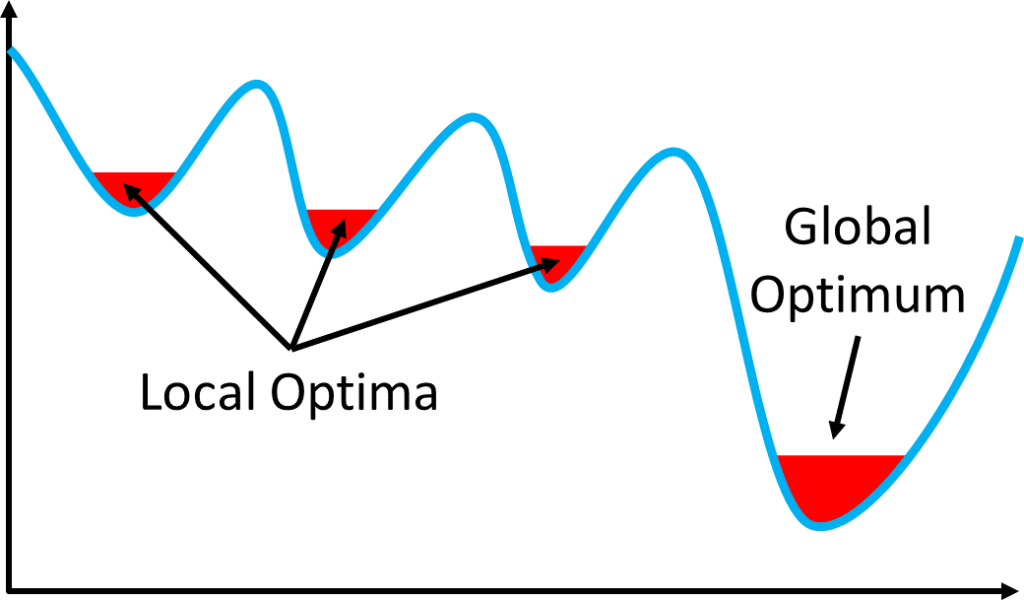
\includegraphics[scale=0.3]{LocalGlobalOptima}
	\centering
	\caption{Full Graph}
\end{figure}

When the greedy algorithm travels down the line,it will continue to do so until it reaches an optima, be that local or global, it does not travel across the whole search space so it easily gets stuck in one of these 'dips' and will not reach the global optimum. In other words by taking the shortest route every time, we may miss a better route which is shorter overall but takes a longer path between some cities. This is much more of an issue for larger search spaces than smaller ones, but since we will be using larger search spaces, it makes this algorithm unsuitable for this experiment.

\subsubsection{Held-Karp Algorithm}
The Held-Karp algorithm is currently the best available for finding the optimum solution with a time complexity of $O(n^2 2^n)$, which whilst not great from a practical stand point, is leagues ahead of its brute force counterpart. This being said with its complexity still being quite high, it is unsuitable for very large datasets as it suffers greatly at these levels, especially so with its inefficient space complexity of $O(n*2^n)$ which is not useful for solving the very large TSP problems without a very high-tech machine on which to run the algorithm, otherwise memory issues can occur as early as 30 city problems \cite{HeldKarpAlg}.

To try and explain the Held-Karp algorithm as simply as possible, it calculates suboptimal shortest paths that satisfy:

\begin{enumerate}
\item Each route must traverse an explicit set of nodes.
\item Each route must end on a specific node.
\end{enumerate}

There is a recursive way of using this algorithm which uses the following formula:
\[cost(x_i, S)=\underset{x_j}{min}\{cost(x_j, S\setminus\{x_i\}) + D_{ji}\}\]
(Credit to: \cite{HeldKarpAlg2})

Where:
\begin{enumerate}
\item $V$ is the set of vertices
\item $D$ is the distance matrix, so $D_{ij}$ is the distance between points $i$ and $j$
\item $S \subset V\setminus\{x_1\} \equiv \{x_2,x_3,...,x_n\}$, $x_i \in S$
\item $cost(x_i,S)$ is the length of the shortest path from $x_1$ to $x_i$ which visits each of the vertices within $S$ exactly once
\item $x_j \in S\setminus\{x_i\}$.
\end{enumerate}


In the case of $S$ having size $1$ we have the base case of:
\[cost(x_i,S) = D_{1i}\]

With this recursive formula we can create the cost function for $S$ for the appropriate sizes, and since it is recursive each step is the basis for the next recursive loop. When we reach the case that $S = V\setminus\{x_1\}$ we have to then find \[\underset{x_i}{min}\{cost(x_i,V\setminus\{x_1\}) + D_{i1}\}\]

with $x_i \in S \equiv V \setminus\{x_1\}$

As stated before even though this is the best for finding the optimal solution to TSP, its time complexity is still exceptionally large and its space complexity also a huge issue. Furthermore for the purposes of this project it is unsuitable since it is already guaranteed to find the optimum,and combining it with any other method will be of no use, only serving to push the time required even further. 

\subsubsection{Christofides Algorithm}
Even with the algorithm having been created over 30 years ago in 1976, there has yet to be another verified algorithm at this time that can produce more optimal approximate solutions to the TSP problem than this. This algorithm has been proven to be at most 50\% worse than the optimal solution whilst having an $O(n^3)$ time complexity where n is the number of cities for which we are trying to solve the problem. \cite{ChrAlg} If we instead look at the best algorithm currently available to solve the TSP (aka the Held-Karp Algorithm) we can see that its complexity is $O(n^2 2^n)$ \cite{HeldKarpAlg} which, whilst astronomically better than the original $O(n!)$, is significantly worse than the approximate solution that Christofides algorithm provides.

This is often the case with such computationally expensive problems, a balance must often be made between finding the optimal solution, and finding a solution in an appropriate amount of time. The Held-Karp algorithm focuses more on finding the optimum answer rather than finding it in a feasible amount of time, whereas Christofides Algorithm was designed to find as best an approximation as it can whilst still having a relatively feasible computation time which is what can make it so appealing to use. 

One of the strong points about Christofides algorithm is just how simple it is, having only 4 or 5 major steps (many sources combine steps 4 and 5 whilst others do not \cite{ChrAlgSlides, ChrAlgSteps}) even if these steps are more likes processes themselves. 

Nonetheless the steps to this algorithm are as follows:
\begin{enumerate}
	\item Find a minimum spanning tree $T$.
	\item Find a minimum weight perfect matching $M$ for the odd degree vertices in $T$.
	\item Calculate $M \bigcup T$.
	\item Find an Euler tour of $M \bigcup T$.
	\item Remove any repeated vertices.
\end{enumerate}

\begin{figure}[ht]
	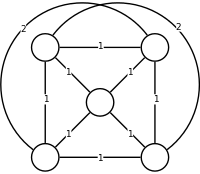
\includegraphics[scale=0.75]{WikiCompleteGraph}
	\centering
	\caption{Full Graph}
\end{figure}

\clearpage
As stated the process is compressed into few steps and is quite simple to understand, and yet creating this algorithm within a programming language is more complex than one would initially assume. Finding a minimum spanning tree (Figure 2) of the full graph (Figure 1) is quite simple, the two most common algorithms known for solving this are Prims and Kruskals, both of which are effective methods with time complexities of $O(n)$ and $O(n^2)$ respectively \cite{PvKTime} though choosing one or the other is mostly affected by the number of edges within the graph we are finding the minimum spanning tree for, with Prims being more suitable if there are a large number of edges, and Kruskals if not.

\begin{figure}[ht]
	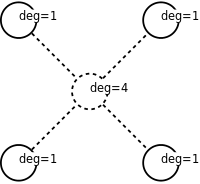
\includegraphics[scale=0.6]{WikiMinSpanTree}
	\centering
	\caption{Minimum Spanning Tree}
\end{figure}

The minimum weight perfect matching of $T$ (Figure 3) is accomplished by finding $\frac{T}{2}$ edges which 'link' together every vertex in $T$ by the shortest edge possible. For this one of the most common algorithm in use appears to be the blossom algorithm and has a time complexity of $O(n^2 m)$ in the worst case where $n$ is the number of vertices and $m$ is the number of edges \cite{BlosAlg}.

\begin{figure}[ht]
	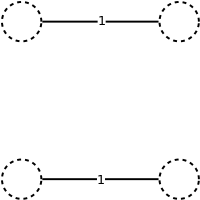
\includegraphics[scale=0.6]{WikiMinMatch}
	\centering
	\caption{Minimum Weight Perfect Matching}
\end{figure}

From here we simply calculate the union of $M$ and $T$ (Figure 4), including any of the repeated edges that may be present, before moving onto the Euler tour. A Euler tour is simply a tour of the graph which visits each edge exactly once, regardless of starting or ending vertex (Figure 5).

\begin{figure}[ht]
	\centering
		\begin{minipage}{0.45\textwidth}
			\centering
			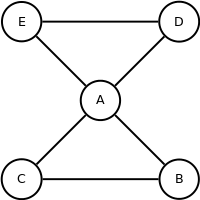
\includegraphics[scale=0.5]{WikiComb}
			\caption{$M \bigcup T$}
		\end{minipage}\hfill
		\begin{minipage}{0.45\textwidth}
			\centering
			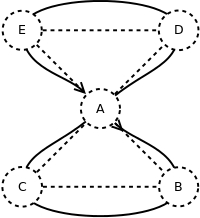
\includegraphics[scale=0.5]{WikiEulerTour}
			\caption{Euler Tour}
		\end{minipage}\hfill
\end{figure}

Then need to remove any repeated vertices within our tour and replace them with the direct edge between those vertices, and once this is done we have the algorithms output (Figure 6).

\begin{figure}[ht]
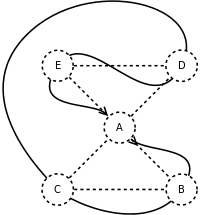
\includegraphics[scale=0.6]{WikiRemove}
\centering
\caption{Christofides Algorithm Output}
\end{figure}

(Figures 1-6 taken from: Wikipedia: Travelling Saleman Problem \cite{TSPWiki})

With this algorithm output we now have a solution to the TSP for our specific graph, and this solution is guaranteed to be within 50\% of the optimum \cite{ChrAlg}, which is significantly better than trying to calculate the true optimum for a very large graph in an infeasible amount of time. However there is clear room for improvement, since for these very large graphs, a solution that is 50\% worse is still drastically longer than the optimum, though is certainly a lot better than the alternative brute force approach. 

This point is either a positive or negative depending on which angle you look at it from. If you look at it from the view that, for a monumental time complexity decrease of $O(n!)$ to $O(n^3)$ you are guaranteed to only be 50\% worse, it looks at it in a positive light, though if you look at it in terms of it being 50\% worse compared to the optimum for very large sets of cities which can have incredibly high distances, it looks quite disadvantageous. I am of the viewpoint that this is a positive thing, as having a solution that is already very good in such a short amount of relative time gives a good basis point for other work to be done with it, exactly as I plan to do within this project.


\begin{thebibliography}{1}

\bibitem{TSPWiki}
Wikipedia: Travelling Salesman Problem
\\\url{https://en.wikipedia.org/wiki/Travelling_salesman_problem} (Accessed 20 October 2020)

\bibitem{HeldKarpAlg}
Hutchinson, C. et al. (no date) ‘CMU Traveling Salesman Problem’, p. 25. Available at: \url{https://www.math.cmu.edu/~af1p/Teaching/OR2/Projects/P58/OR2_Paper.pdf} (Accessed: 27 October 2020)

\bibitem{HeldKarpAlg2}
Nguyen, Q. N. (no date) ‘Travelling Salesman Problem and Bellman-Held-Karp Algorithm’, p. 5. Available at: \url{http://www.math.nagoya-u.ac.jp/~richard/teaching/s2020/Quang1.pdf} (Accessed: 12 November 2020)

\bibitem{TSP2020}
Klarreich, E. (no date) Computer Scientists Break Traveling Salesperson Record, Quanta Magazine. Available at: \url{https://www.quantamagazine.org/computer-scientists-break-traveling-salesperson-record-20201008/} (Accessed: 22 October 2020).

\bibitem{ChrAlg}
Christofides, N. (1976) Worst-Case Analysis of a New Heuristic for the Travelling Salesman Problem. CARNEGIE-MELLON UNIV PITTSBURGH PA MANAGEMENT SCIENCES RESEARCH GROUP. Available at: \url{https://apps.dtic.mil/sti/citations/ADA025602} (Accessed: 22 October 2020).

\bibitem{ChrAlgSlides}
Sitters, R. (no date) Chapter 2: Greedy Algorithms and Local Search. Available at: \url{https://personal.vu.nl/r.a.sitters/AdvancedAlgorithms/2016/SlidesChapter2-2016.pdf} (Accessed: 27 October 2020).

\bibitem{ChrAlgSteps}
Christofides algorithm (no date). Available at: \url{https://xlinux.nist.gov/dads/HTML/christofides.html} (Accessed: 27 October 2020).

\bibitem{PvKTime}
Huang, F., Gao, P. and Wang, Y. (2009) ‘Comparison of Prim and Kruskal on Shanghai and Shenzhen 300 Index Hierarchical Structure Tree’, in 2009 International Conference on Web Information Systems and Mining. 2009 International Conference on Web Information Systems and Mining, pp. 237–241. doi: 10.1109/WISM.2009.56.

\bibitem{BlosAlg}
Kolmogorov, V. (2009) ‘Blossom V: a new implementation of a minimum cost perfect matching algorithm’, Mathematical Programming Computation, 1(1), pp. 43–67. doi: 10.1007/s12532-009-0002-8.
Available at: \url{http://mpc.zib.de/archive/2009/1Kolmogorov2009_Article_BlossomVANewImplementationOfAM.pdf} (Accessed: 29 October 2020)

\bibitem{GAIntro}
Melanie, M. (no date) ‘An Introduction to Genetic Algorithms’, p. 162. Available at: \url {http://www.boente.eti.br/fuzzy/ebook-fuzzy-mitchell.pdf} (Accessed: 3 November 2020)

\bibitem{TSPGACrMu}
Penev, M.K.V.S.S., 2005. Genetic operators crossover and mutation in solving the TSP problem. In International Conference on Computer Systems and Technologies. Available at: \url{http://citeseerx.ist.psu.edu/viewdoc/download?doi=10.1.1.83.7264&rep=rep1&type=pdf} (Accessed: 5 November 2020)

\bibitem{GAMutations}
Abdoun, O., Abouchabaka, J. and Tajani, C. (no date) ‘Analyzing the Performance of Mutation Operators to Solve the Travelling Salesman Problem’, p. 18. Available at: \url{https://arxiv.org/pdf/1203.3099.pdf} (Accessed: 5 November 2020)

\bibitem{GACrossover}
Hussain, A. et al. (2017) ‘Genetic Algorithm for Traveling Salesman Problem with Modified Cycle Crossover Operator’, Computational Intelligence and Neuroscience, 2017, pp. 1–7. doi: 10.1155/2017/7430125. Available at: \url{http://downloads.hindawi.com/journals/cin/2017/7430125.pdf} (Accessed: 10 November 2020)

\bibitem{GACrossoverPerformance}
Otman, A. (no date) ‘A Comparative Study of Adaptive Crossover Operators for Genetic Algorithms to Resolve the Traveling Salesman Problem’, International Journal of Computer Applications, 31, p. 9.
Available at: \url{https://arxiv.org/pdf/1203.3097.pdf} (Accessed: 12 November 2020)

\bibitem{TSPRep1}
TSP Test Data (no date). Available at: http://www.math.uwaterloo.ca/tsp/data/index.html (Accessed: 12 November 2020).

\bibitem{TSPRep2}
TSPLIB (no date). Available at: http://comopt.ifi.uni-heidelberg.de/software/TSPLIB95/ (Accessed: 12 November 2020).

\bibitem{DiffAlgs}
Baidoo, E. and O., S. (2016) ‘Solving the TSP using Traditional Computing Approach’, International Journal of Computer Applications, 152(8), pp. 13–19. doi: 10.5120/ijca2016911906. Available at: \url{https://www.researchgate.net/profile/Evans_Baidoo2/publication/309224559_Solving_the_TSP_using_Traditional_Computing_Approach/links/58066b6408ae5ad188166189.pdf} (Accessed: 12 November 2020)



\end{thebibliography}

\begin{appendices}
\end{appendices}

\end{document}